Trattiamo di seguito l'elaboratore delle interrogazioni.
\begin{figure}[h]
    \centering
    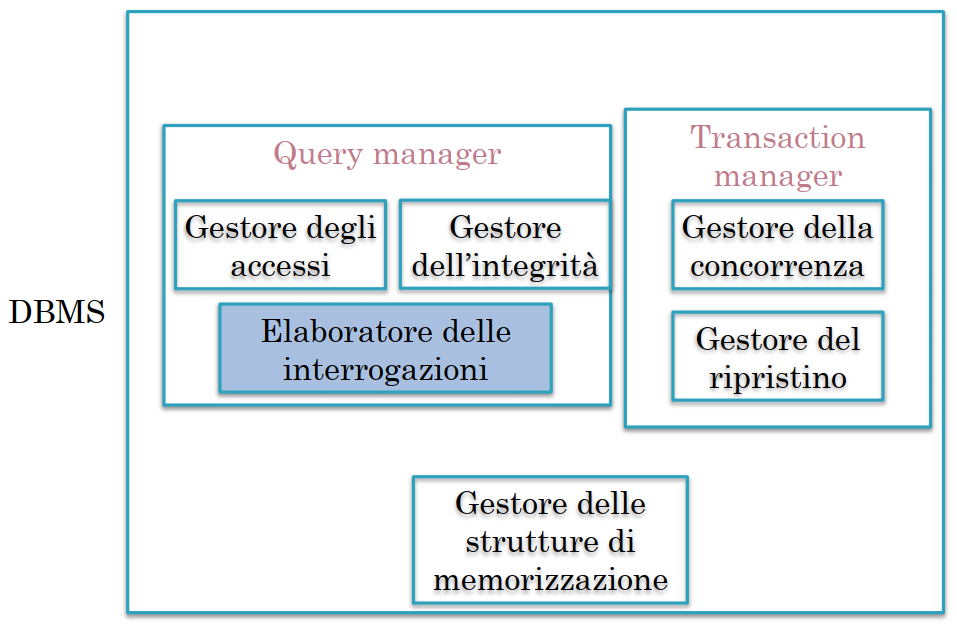
\includegraphics[width=0.8\textwidth, keepaspectratio]{componenti2.png}
    \label{fig:componenti2}
\end{figure}
L'ottimizzazione logica \`e la scelta del piano logico più efficiente. Seppur costosa, il guadagno che ne otteniamo ne vale a pena.\\
Query di esempio:\\
\code{SELECT B,D\\
FROM R,S\\
WHERE R.A = "c" AND S.E = 2 AND R.C=S.C}

\begin{figure}[htbp]
    \centering
    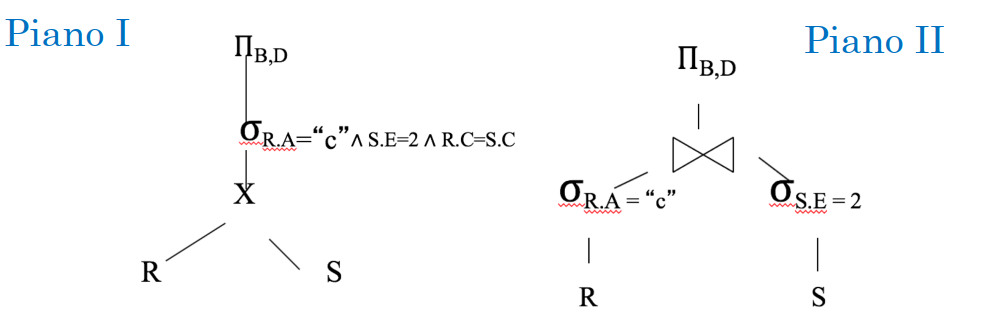
\includegraphics[width=0.8\textwidth, keepaspectratio]{pianiLogici.png}
    \caption{Possibili piani logici per la query di esempio}
    \label{fig:pianiLogici}
\end{figure}
Da questi piani possiamo quindi trovare un piano fisico a seconda degli indici presenti e strutture dei file.\\
L'esecuzione di una query si può dividere in parti:
\begin{figure}[htbp]
    \centering
    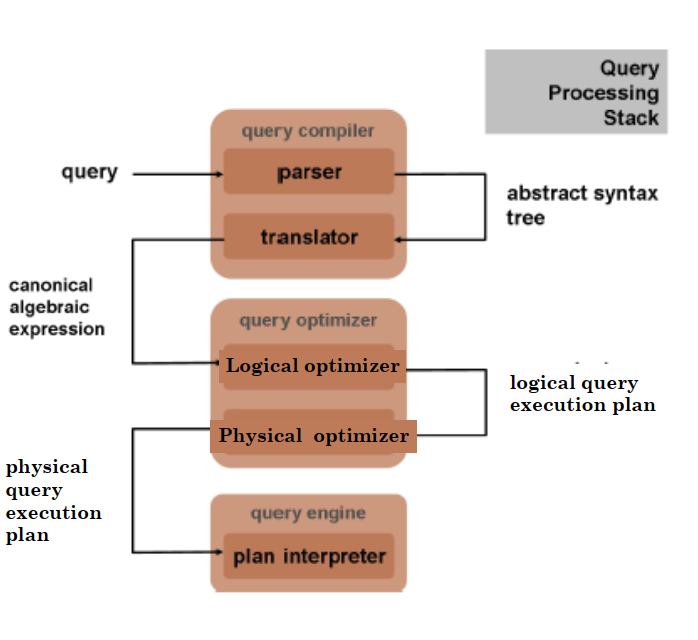
\includegraphics[width=0.8\textwidth, keepaspectratio]{queryProcessing.png}
    \label{fig:queryProcessing}
\end{figure}

\break

\subsection{Ottimizzatore logico}
\begin{itemize}
    \item \textbf{input}: espressione algebrica canonica
    \item \textbf{output}: piano di esecuzione logico ottimizzato (albero)
\end{itemize}
Basata su equivalenze algebriche.\\
Vengono seguite delle regole di riscrittura per applicare le equivalenze ed ottenere un'espressione equivalente ma più efficiente.\\
\begin{definition} \textbf{Equivalenze Algebriche}: Due espressioni e1 ed e2 dell'algebra relazionale sono dette equivalenti se, per ogni possibile base di dati in input D, producono lo stesso risultato in output quando vengono eseguite su D
\end{definition}
\begin{figure}[htbp]
    \centering
    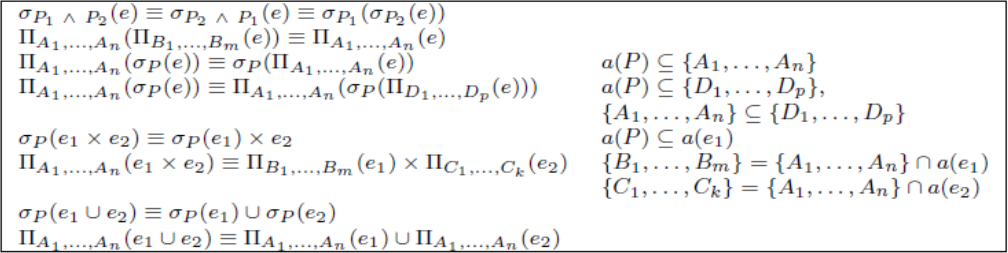
\includegraphics[width=\textwidth, keepaspectratio]{equivalenzeAlgebriche.png}
    \label{fig:equivalenzeAlgebriche}
\end{figure}
Inoltre abbiamo anche:
\begin{itemize}
    \item Commutatività e associatività di join e prodotto cartesiano
    \item relazioni tra join, prodotto Cartesiano e selezione
\end{itemize}

\subsubsection{Regole di riscrittura}
Principi base:
\begin{itemize}
    \item Anticipare il più possibile le operazioni che permettono di ridurre la dimensione dei risultati intermedi (selezione e proiezione)
    \item Fattorizzare condizioni di selezione complesse e lunghe liste di attributi in proiezioni, per aumentare la possibilità di applicare regole di riscrittura
\end{itemize}
\textbf{L'ordine di esecuzione dei join} viene scelto nella fase successiva (ottimizzazione fisica).\\
Euristiche:
\begin{enumerate}
    \item Eseguire le operazioni di selezione ($\sigma$) il più presto possibile
    \item Eseguire le operazioni di proiezione ($\Pi$) il più presto possibile
    \item Introdurre ulteriori proiezioni nell’espressione, gli unici attributi da non eliminare sono quelli che appaiono nel risultato della query oppure sono necessari in operazioni successive.
\end{enumerate}

\subsection{Ottimizzatore fisico}
\begin{itemize}
    \item \textbf{input}: piano di esecuzione logico ottimizzato (albero)
    \item \textbf{output}: piano di esecuzione fisico ottimale (algoritmo rappresentato come albero)
\end{itemize}
\`E importante determinare la dimensione fisica dei risultati di ogni operatore siccome saranno poi l'input dell'operatore successivo.\\
In questa fase si scelgono anche:
\begin{itemize}
    \item Eventuali nodi aggiuntivi per operazioni che ottimizzerebbero delle esecuzioni (ad esempio ordinamento)
    \item Un ordine di esecuzione
    \item Come passare i dati da un operatore all'altro
\end{itemize}

\begin{figure}[htbp]
    \centering
    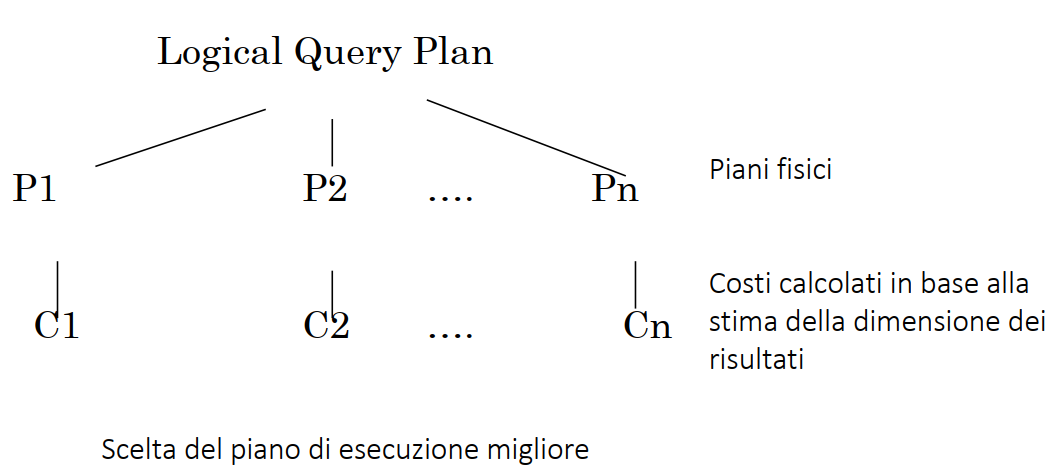
\includegraphics[width=0.8\textwidth, keepaspectratio]{pianiFisici.png}
    \label{fig:pianiFisici}
\end{figure}

\subsection{Esecuzione del piano}
\begin{itemize}
    \item \textbf{input}: piano di esecuzione fisico ottimale
    \item \textbf{output}: risultato
\end{itemize}